%% LyX 2.3.5.2 created this file.  For more info, see http://www.lyx.org/.
%% Do not edit unless you really know what you are doing.
\documentclass[british]{article}
\usepackage[T1]{fontenc}
\usepackage[latin9]{inputenc}
\usepackage{geometry}
\geometry{verbose,lmargin=1cm,rmargin=1cm}
\usepackage{refstyle}
\usepackage{amsmath}
\usepackage{amsthm}
\usepackage{amssymb}
\usepackage{cancel}
\usepackage{graphicx}
\PassOptionsToPackage{normalem}{ulem}
\usepackage{ulem}

\makeatletter

%%%%%%%%%%%%%%%%%%%%%%%%%%%%%% LyX specific LaTeX commands.

\AtBeginDocument{\providecommand\Eqref[1]{\ref{Eq:#1}}}
\AtBeginDocument{\providecommand\Figref[1]{\ref{Fig:#1}}}
\AtBeginDocument{\providecommand\Algref[1]{\ref{Alg:#1}}}
\AtBeginDocument{\providecommand\Lemref[1]{\ref{Lem:#1}}}
\AtBeginDocument{\providecommand\Defref[1]{\ref{Def:#1}}}
\AtBeginDocument{\providecommand\Remref[1]{\ref{Rem:#1}}}
\RS@ifundefined{subsecref}
  {\newref{subsec}{name = \RSsectxt}}
  {}
\RS@ifundefined{thmref}
  {\def\RSthmtxt{theorem~}\newref{thm}{name = \RSthmtxt}}
  {}
\RS@ifundefined{lemref}
  {\def\RSlemtxt{lemma~}\newref{lem}{name = \RSlemtxt}}
  {}


%%%%%%%%%%%%%%%%%%%%%%%%%%%%%% Textclass specific LaTeX commands.
\numberwithin{equation}{section}
\numberwithin{figure}{section}
\theoremstyle{plain}
\newtheorem{thm}{\protect\theoremname}
\theoremstyle{definition}
\newtheorem{defn}[thm]{\protect\definitionname}
\theoremstyle{plain}
\newtheorem{lyxalgorithm}[thm]{\protect\algorithmname}
\theoremstyle{plain}
\newtheorem{lem}[thm]{\protect\lemmaname}
\theoremstyle{remark}
\newtheorem{rem}[thm]{\protect\remarkname}

%%%%%%%%%%%%%%%%%%%%%%%%%%%%%% User specified LaTeX commands.
%\newref{thm}{name=theorem~,Name=Theorem~,names=theorems~,Names=Theorems~}
\newref{def}{name=definition~,Name=Definition~,names=definitions~,Names=Definitions~}
%\newref{cor}{name=corollary~,Name=Corollary~,names=corollaries~,Names=Corollaries~}
\newref{lem}{name=lemma~,Name=Lemma~,names=lemmas~,Names=Lemmas~}
%\newref{claim}{name=claim~,Name=Claim~,names=claims~,Names=Claims~}
%\newref{sec}{name=section~,Name=Section~,names=sections~,Names=Sections~}
%\newref{subsec}{name=subsection~,Name=Subsection~,names=subsections~,Names=Subsections~}
%\newref{prop}{name=proposition~,Name=Proposition~,names=propositions~,Names=Propositions~}
%\newref{conj}{name=conjecture~,Name=Conjecture~,names=conjectures~,Names=Conjectures~}
%\newref{conj}{name=conjecture~,Name=Conjecture~,names=conjectures~,Names=Conjectures~}
\newref{rem}{name=remark~,Name=Remark~,names=remarks~,Names=Remarks~}
\newref{eq}{name=equation~,Name=Equation~,names=equations~,Names=Equations~}
\newref{alg}{name=algorithm~,Name=Algorithm~,names=algorithms~,Names=Algorithms~}

\makeatother

\usepackage{babel}
\providecommand{\algorithmname}{Algorithm}
\providecommand{\definitionname}{Definition}
\providecommand{\lemmaname}{Lemma}
\providecommand{\remarkname}{Remark}
\providecommand{\theoremname}{Theorem}

\begin{document}
\title{Local and Robust Self testing using trapped ions}
\author{Xiaomin etc.., Atul Singh Arora, Kishor Bharti, Adan Cabello, Kwek
Leong Chuan}
\maketitle
\begin{abstract}
We provide experimental implementation of KCBS self-testing scheme.
Theoretical tools are supplemented to render the results in \textit{Physical
Review Letters 122 (25), 250403 }practical.
\end{abstract}

\section{Introduction}

\subsection{Why self-testing}

\subsubsection{State of the art}
\begin{itemize}
\item Bell/Device independence | Tensor structure
\begin{itemize}
\item Limitation: Difficult to enforce etc
\item Curve less robust to noise
\item Math is harder
\end{itemize}
\item Semi device independent
\begin{itemize}
\item Easier to implement
\item EPR steering {[}K{]}; almost like blind computing
\end{itemize}
\item All bipartite entangled states can be self-tested by quantum steering
| EPR steering
\end{itemize}

\subsubsection{Local Self testing }

Motivation: Device certification.
\begin{itemize}
\item Computation, which is usually local, it is inconvenient also less
secure to trust another party etc.
\end{itemize}
State of the art
\begin{itemize}
\item Vidick et al
\item Kishor's et al article on self-testing. Robustness curve was given
up to multiplicative constants. Not directly implementable. 
\end{itemize}

\subsubsection{Contextuality}

Informal quick introduction

\subsubsection{Contribution}

Address limitations of Kishor et al's article
\begin{itemize}
\item theoretically obtained the robustness curve
\begin{itemize}
\item Moment matrices based approach
\item First robustness curve for a non-contextuality inequality (five cycles
no less!)
\end{itemize}
\item experimental demonstration of local self-testing
\end{itemize}

\subsubsection{Assumptions and Memory leakage :P}

Self testing works under the following.

\subsubsection{Circumventing the memory assumption}
\begin{itemize}
\item Memory based
\begin{itemize}
\item Quantum classical gap?
\end{itemize}
\item Dimensions based measures
\begin{itemize}
\item Quantum classical gap 
\item log{[}classical dimensions{]}=memory; quantum dimension = quantum
memory
\end{itemize}
\end{itemize}
Criticism:

BQP$\subseteq$PSPACE; that's fine we hope to find the exact curve
to certify
\begin{itemize}
\item Poly separation or some such.
\end{itemize}

\section{Background}

\subsection{Exclusivity graph approach to contextuality}

\subsection{Robust self-testing}
\begin{itemize}
\item Definition
\item Statement for KCBS {[}PRL{]}
\item Robustness curve is missing! Or is it?
\end{itemize}


\section{Robustness Curve}

{[}DISCLAIMER: I am writing the following as rough notes which may
ramble but should at least be consistent; in the following iteration,
I hope to make improve the presentation{]}

What we have is some experimental data

\subsection{Description}

\global\long\def\KCBS{\text{KCBS}}%

\global\long\def\tr{\text{tr}}%

TODO:
\begin{itemize}
\item IID
\item Restricted subspace or full subspace, Bell
\item Parallel or Serial
\begin{itemize}
\item When IID, parallel and serial should become identical
\item When not IID, parallel should be more general
\end{itemize}
\item Clarify the issue with the sum
\item NOTATIONAL
\begin{itemize}
\item Difference between a ``configuration'' and a ``realisation''.
\end{itemize}
\end{itemize}
\begin{defn}[Experimental Scenario]
\end{defn}

\begin{defn}[Quantum Realisation]
\end{defn}

Consider the KCBS scenario, i.e. an experimental scenario which is
specified by the events $e_{1},e_{2}\dots e_{5}$ whose exclusivity
is given by a $5$-cycle exclusivity graph. Suppose we obtain the
probabilities $p_{1},p_{2}\dots p_{5}$ experimentally (and ensure
that they correspond to sharp measurements). We already saw that if
these values nearly saturate the quantum bound for the KCBS non-contextuality
inequality, i.e. $\sum_{i=1}^{5}p_{i}$ approaches $\sqrt{5}\approx2.236\dots$,
then we know that all quantum realisations corresponding to the experimentally
obtained probabilities $\{p_{i}\}_{i=1}^{5}$ are almost equivalent
to $\rho^{\text{KCBS}},\{\Pi_{i}^{\text{KCBS}}\}_{i=1}^{5}$, up to
a global isometry. To be more precise, consider any arbitrary quantum
realisation given by a pure state $\rho$ and rank one projectors
$\{\Pi_{i}\}$ such that $\sum_{i=1}^{5}p_{i}=2+\epsilon$. It was
shown in \cite{Bharti2018} that then, there exists an isometry $V$
such that 
\begin{equation}
\left\Vert V\Pi_{i}V^{\dagger}-\Pi_{i}^{\KCBS}\right\Vert _{F}\le\mathcal{O}(\sqrt{\epsilon})\label{eq:projKish}
\end{equation}
 for all $i\in\{1,2\dots5\}$ and $\left\Vert \rho-\rho^{{\rm KCBS}}\right\Vert _{F}\le\mathcal{O}(\sqrt{\epsilon})$
where $\left\Vert A\right\Vert _{F}:={\rm tr}\left(\sqrt{A^{\dagger}A}\right)$.
Despite this, without the constant hidden in \Eqref{projKish}, one
cannot obtain a robustness curve and thus one cannot apply this in
practice. In this work, we remedy this problem, taking inspiration
from the Bell self-testing approach. To this end, we give a slightly
different statement: we show that
\begin{equation}
\sum_{i=1}^{5}\mathcal{F}(V\Pi_{i}\rho\Pi_{i}V^{\dagger},\Pi_{i}^{\KCBS}\rho^{\KCBS}\Pi_{i}^{\KCBS})+\mathcal{F}(V\rho V^{\dagger},\rho^{\KCBS})\ge f(\epsilon)\label{eq:lowerbound}
\end{equation}
 where $\mathcal{F}(A,B):={\rm tr}\sqrt{\left|A^{1/2}B^{1/2}\right|}$,
we only require $\Pi_{i}$ to be projectors (such that $[\Pi_{i},\Pi_{j}]=0$
if $(i,j)$ is an edge of the exclusivity graph) and allow $\rho$
to be a mixed state. The advantage is that we are able to express
$f(\epsilon)$ as a hierarchy of semi-definite programmes and compute
lower bounds explicitly. While we state our result for the KCBS inequality,
it readily extends to the $n$-cycle scenario. {[}TODO: if $f$ cannot
be shown to be independent of the individual $p_{i}$s, then we must
skip it{]}. 


\subsection{Overall Strategy}
\begin{defn}[An ideal KCBS configuration]
Consider a three-dimensional Hilbert space spanned by the basis $\{\left|0\right\rangle ,\left|1\right\rangle ,\left|2\right\rangle \}$.
Let 
\[
\left|u_{l}\right\rangle :=\cos\theta\left|0\right\rangle +\sin\theta\sin\phi_{l}\left|1\right\rangle +\sin\theta\cos\phi_{l}\left|2\right\rangle 
\]
 where $\phi_{l}:=l\pi(n-1)/n$ for $1\le l\le n$. Define 
\begin{align*}
\left|\psi^{\KCBS}\right\rangle  & :=\left|0\right\rangle \\
\Pi_{i}^{\KCBS} & :=\left|u_{i}\right\rangle \left\langle u_{i}\right|.
\end{align*}
\end{defn}

TODO
\begin{itemize}
\item \sout{Verify if we require that \mbox{$\Pi_{i}\Pi_{j}=0$} or that
\mbox{$\tr[\Pi_{i}\Pi_{j}\rho]=0$}. \mbox{$\tr[\Pi_{i}\Pi_{j}\Pi_{k}\rho]$}
(by assumption; write clearly in the previous section); {[}status:
we handled this already{]}}
\item Update: say that $\rho=\left|\psi\right\rangle \left\langle \psi\right|$
without loss of generality
\end{itemize}
We may restate the aforesaid discussion more symbolically as lower
bounding the value of the following objective function: 
\begin{equation}
F:=\min_{\rho,\{\Pi_{i}\}}\max_{V}\left[\sum_{i=1}^{5}\mathcal{F}(V\Pi_{i}\rho\Pi_{i}V^{\dagger},\Pi_{i}^{\KCBS}\rho^{\KCBS}\Pi_{i}^{\KCBS})+\mathcal{F}(V\rho V^{\dagger},\rho^{\KCBS})\right]\label{eq:fidelity}
\end{equation}
where $\rho,\{\Pi_{i}\}_{i=1}^{5}$ is a quantum realisation\footnote{note that we assume $\Pi_{i}$ are projectors as the measurements
are assumed to be sharp experimentally} of $\{p_{i}\}_{i=1}^{5}$, $V$ is an isometry from $\mathcal{H}$
to $\mathcal{H}^{\KCBS}$, i.e. from the space on which $\rho,\{\Pi_{i}\}_{i=1}^{5}$
act/are defined to that where $\rho^{\KCBS},\{\Pi_{i}^{\KCBS}\}_{i=1}^{5}$
act/are defined. At the broadest level, the idea is to drop the maximization
over $V$ and replace it with a particular isometry $V$ which is
expressed in terms of $\rho,\{\Pi_{i}\}_{i=1}^{5}$. Then, as we shall
see, the expression for the fidelity appears as a sum of terms of
the following form. Let $w$ be a word created from the letters, $\{\mathbb{I},\Pi_{1},\Pi_{2}\dots\Pi_{5},\hat{P}\}$
with $\hat{P}^{\dagger}\hat{P}=\mathbb{I}$, $\Pi_{i}^{2}=\Pi_{i}$
and $\Pi_{i}\Pi_{j}=0$ if $(i,j)\in E(G)$, i.e. when $i,j$ are
exclusive\footnote{We introduced $\hat{P}$ for completeness; its role is explained later.}.
The fidelity is a linear combination of these words, i.e. $F=\min_{\left\{ \left\langle w\right\rangle \right\} }\sum_{w}\alpha_{w}\left\langle w\right\rangle $
where $\tr[w\rho]=:\left\langle w\right\rangle $, subject to the
constraint that $\{\left\langle w\right\rangle \}_{w}$ corresponds
to a quantum realisation. The advantage of casting the problem in
this form is that one can now construct an NPA-like hierarchy. The
idea is simple to state. Treat $\left\{ \left\langle w\right\rangle \right\} _{w}$
as a vector. Denote by $Q$ the set of all such vectors which correspond
to a quantum realisation (of $\left\{ p_{i}\right\} _{i=1}^{5}$).
It turns out that one can impose constraints on words with $k$ letters,
for instance. Under these constraints, denote by $Q_{k}$ the set
that is obtained. Note that $Q_{k}\supseteq Q$ for it may contain
vectors which don't correspond to the quantum realisation. In fact,
$Q_{k}$ can be characterised using semi-definite programming constraints
(which in turn means they are efficiently computable). Intuitively,
it is clear that $\lim_{k\to\infty}Q_{k}=Q$. Further, it is also
clear that $F=\min_{\{\left\langle w\right\rangle \}_{w}\in Q}\sum_{w}\alpha_{w}\left\langle w\right\rangle \ge\min_{\left\{ \left\langle w\right\rangle \right\} _{w}\in Q_{k}}\sum_{w}\alpha_{w}\left\langle w\right\rangle $
as we are minimising over a larger set on the right hand side. 

\subsection{Providing a lower bound on the fidelity from regularized measurement
statistics}
\begin{itemize}
\item TODO
\begin{itemize}
\item \sout{{[}done{]} To conclude that \mbox{$\sum_{k=0}^{n-1}\left|k\right\rangle \left\langle k\right|\otimes P^{-k}$}
is an isometry, we need to assume rank one projectors. }
\item $\mathcal{G}$
\end{itemize}
\end{itemize}
\global\long\def\swap{{\rm SWAP}}%

For concreteness, we first consider a unitary $U_{\swap}$ instead
of an isometry, which acts on two spaces $\mathcal{A}$ and $\mathcal{A}'$.
For simplicity, suppose that the $\mathcal{A}$ register is in the
state 
\[
\sigma\in\underbrace{\{\left|\psi^{\KCBS}\right\rangle \left\langle \psi^{\KCBS}\right|\}\cup\{\Pi_{i}^{\KCBS}\}_{i=1}^{5}}_{:=\mathcal{S}^{\KCBS}}.
\]
We want $U_{\swap}$ to map $\sigma_{\mathcal{A}}\otimes\left|0\right\rangle \left\langle 0\right|_{\mathcal{A}'}$
to $\left|0\right\rangle \left\langle 0\right|_{\mathcal{A}}\otimes\sigma_{\mathcal{A}'}$
(see \Figref{IllustrationSWAP}). Our strategy is to construct $U_{\swap}$
in this seemingly trivial case and then express it in terms of the
state and measurement operators on $\mathcal{A}$. The rationale is
that by construction, $U_{\swap}$ will work for the ideal case and
therefore should also work for cases close to ideal. This should become
clear momentarily. Note that any circuit that swaps two qutrits should
let us achieve our simplified goal (because all elements of $S^{\KCBS}$
are defined on a three dimensional Hilbert space). One possible qutrit
swapping unitary/circuit (a special case of the general qudit swapping
unitary/circuit defined in {[}??{]}, an article about self-testing
Bell inequalities) may be defined as $S_{\swap}'':=TUVU$ where 

\begin{align}
T & :=\mathbb{I}_{\mathcal{A}}\otimes\sum_{k=0}^{2}\left|-k\right\rangle \left\langle k\right|_{\mathcal{A}'}\nonumber \\
U & :=\sum_{k=0}^{2}P_{\mathcal{A}}^{k}\otimes\left|k\right\rangle \left\langle k\right|_{\mathcal{A}'}\nonumber \\
V & :=\sum_{k=0}^{2}\left|\bar{k}\right\rangle \left\langle \bar{k}\right|_{\mathcal{A}}\otimes P_{\mathcal{A}'}^{-k}\label{eq:TUV}
\end{align}
where $P:=\sum_{i=0}^{2}\left|\overline{k+1\mod3}\right\rangle \left\langle \bar{k}\right|$
is a translation operator and $\{\left|\bar{0}\right\rangle ,\left|\bar{1}\right\rangle ,\left|\bar{2}\right\rangle \}$
is a basis for the qutrit space {[}TODO: fix the bar issue{]}. We
omit the proof here (for a proof see ...). To generalise this idea
and to construct an isometry, we relax the assumption that $\mathcal{A}$
is a three dimensional Hilbert space. We re-express/replace the operations
in $T,U,V$ which act on the $\mathcal{A}$ space by linear combinations
of monomials in $\{\Pi_{i}\}_{i=1}^{5}$. We obtain the coefficients
used in these linear combinations by assuming the space is three dimensional.
The idea is simply that this map reduces to a swap operation when
we re-impose the assumptions and for cases close to it, we expect
it to behave appropriately. (TODO: maybe add the circuit for bell
inequality to explain at some point?) We describe this procedure more
precisely below. 
\global\long\def\cross{\text{cross}}%

\begin{lyxalgorithm}[Constructing an isometry]
 Let\label{alg:ConstructingAnIsometry}
\begin{itemize}
\item $\mathcal{A}'$ be a three dimensional Hilbert space spanned by an
orthonormal basis $\left\{ \left|0\right\rangle _{\mathcal{A}'},\left|1\right\rangle _{\mathcal{A}'},\left|2\right\rangle _{\mathcal{A}'}\right\} $,
\item $\rho^{\KCBS},\{\Pi_{i}^{\KCBS}\}_{i=1}^{5}$ be an ideal quantum
realisation (see ...) on $\mathcal{A}'$,
\item $\mathcal{A}$ be a Hilbert space with dimension at least $3$ containing
orthonormal vectors $\left\{ \left|\bar{0}\right\rangle _{\mathcal{A}},\left|\bar{1}\right\rangle _{\mathcal{A}},\left|\bar{2}\right\rangle _{\mathcal{A}}\right\} $
\item $\rho,\{\Pi_{i}\}_{i=1}^{5}$ be an arbitrary quantum realisation
on defined on $\mathcal{A}$. 
\end{itemize}
Define $T,U,V$ as in \Eqref{TUV} and let $S'_{\swap}:=TUVU$ with
the following changes. Let 
\[
\mathcal{W}^{\KCBS}:=\{\{\Pi_{i}^{\KCBS}\}_{i=1}^{5},\{\Pi_{i}^{\KCBS}\Pi_{j}^{\KCBS}\}_{i,j=1}^{5},\dots\}
\]
 and 
\[
\mathcal{W}:=\{\{\Pi_{i}\}_{i=1}^{5},\{\Pi_{i}\Pi_{j}\}_{i,j=1}^{5}\dots\}
\]
 be the set of ``words'' formed by the KCBS projectors and those
of the arbitrary quantum realisation, respectively.
\begin{enumerate}
\item Translation Operator: 
\begin{enumerate}
\item Express $P_{\mathcal{A}'}$ as a linear combination of elements in
$\mathcal{W}$, i.e. $P_{\mathcal{A}'}=\sum_{l^{\KCBS}\in\mathcal{W}^{\KCBS}}\alpha_{l}l^{\KCBS}$.
\item Define $P_{\mathcal{A}}:=\sum_{l\in\mathcal{W}}\alpha_{l}l$
\end{enumerate}
\item Basis projectors: Formally replace, in $V$, the operators 
\begin{enumerate}
\item $\left|\bar{0}\right\rangle \left\langle \bar{0}\right|_{\mathcal{A}}$
by $\Pi_{1}$,
\item $\left|\bar{1}\right\rangle \left\langle \bar{1}\right|_{\mathcal{A}}$
by $\Pi_{2}$ and, 
\item $\left|\bar{2}\right\rangle \left\langle \bar{2}\right|_{\mathcal{A}}$
by $(\mathbb{I}-\Pi_{1})(\mathbb{I}-\Pi_{2})$
\end{enumerate}
i.e. $V$ now becomes $\Pi_{1}\otimes\mathbb{I}_{\mathcal{A}'}+\Pi_{2}\otimes P_{\mathcal{A}'}^{-1}+(\mathbb{I}-\Pi_{1})(\mathbb{I}-\Pi_{2})\otimes P_{\mathcal{A}'}^{-2}$. 
\end{enumerate}
\end{lyxalgorithm}

We do not prove but {[}{*}{*}CHECK{]} it is known that the linear
combinations required in \Algref{ConstructingAnIsometry} always exist,
i.e. the algorithm always succeeds at constructing $S'_{\swap}$.
We must show that $S'_{\swap}$ is in fact an isometry. This is important
because of the following reason. Recall that our objective was to
lower bound \Eqref{fidelity}. To this end, we said we drop the maximization
over all possible $V$s, (for a given quantum realisation $\rho,\left\{ \Pi_{i}\right\} _{i=1}^{5}$)
and instead insert a specific isometry $S'_{\swap}$ (which is a function
of $\rho,\{\Pi_{i}\}_{i=1}^{5}$). Note that this argument for lower
bounding \Eqref{fidelity} breaks if $S'_{\swap}$ is not an isometry.
In fact, $P_{\mathcal{A}}$ as produced by the algorithm is not necessarily
unitary (viz. $P_{\mathcal{A}}^{\dagger}P_{\mathcal{A}}=\mathbb{I}_{\mathcal{A}}$
may not hold). Following {[}??{]} we use the so-called localising
matrix technique, which we discuss in some detail later. We introduce
a new unitary matrix $\hat{P}_{\mathcal{A}}$ satisfying $\hat{P}P\ge0$
where we dropped the subscript for clarity. Consider the case where
$P$ is not unitary. In that case, one can use polar decomposition
to write $P=\left|P\right|U$ (not to be confused with the $U$ above;
where $\left|P\right|\ge0$ and $U^{\dagger}U=\mathbb{I}$) so choosing
$\hat{P}=U^{\dagger}$ satisfies $\hat{P}P\ge0$. Thus for each $P$,
the constraint can be satisfied. Consider the other case, i.e. where
$P=U$ is unitary. Then,\footnote{{[}TODO: verify the reasoning once again{]} To see this, write the
polar decomposition of $\hat{P}=\left|\hat{P}\right|E$ (where $\left|\hat{P}\right|\ge0$
and $E^{\dagger}E=\mathbb{I}$). Then $\hat{P}U=\left|\hat{P}\right|EU$
which is a polar decomposition of $\hat{P}U$. The polar decomposition
of a positive semi-definite matrix $M$ always has the form $M.\mathbb{I}$.
Using $M=\hat{P}U$, and identifying $EU$ with $\mathbb{I}$, we
have $E=U^{\dagger}$. } $\hat{P}=U^{\dagger}$. Thus, in the ideal case we recover the same
unitary and for the case close to ideal, we are guaranteed that there
is some solution (which we expect should also work reasonably). Combining
these, we can construct $U_{\swap}$ which is an isometry.
\begin{lem}[$U_{\swap}$ is indeed an Isometry]
 Let $S'_{\swap}$ be the map produced by \Algref{ConstructingAnIsometry}
and define $S_{\swap}$ to be $S'_{\swap}$ with $P_{\mathcal{A}}$
replaced by $\hat{P}_{\mathcal{A}}$. Then $S_{\swap}$ is an isometry
if the following conditions hold \label{lem:UswapIsAnIsometry}
\begin{align*}
\hat{P}_{\mathcal{A}}^{\dagger}\hat{P}_{\mathcal{A}} & =\mathbb{I}_{\mathcal{A}},\\
\hat{P}_{\mathcal{A}}P_{\mathcal{A}} & \ge0.
\end{align*}
\end{lem}

\begin{proof}
It suffices to show that $\left\langle \psi\right|_{\mathcal{A}'\mathcal{A}}S_{\swap}^{\dagger}S_{\swap}\left|\psi\right\rangle _{\mathcal{A}'\mathcal{A}}=1$
for all normalised $\left|\psi\right\rangle _{\mathcal{A}'\mathcal{A}}$.
We express $S_{\swap}=TUVU$ where $T$ is as in \Eqref{TUV}, $U:=\sum_{k=0}^{2}\hat{P}_{\mathcal{A}}^{k}\otimes\left|\bar{k}\right\rangle \left\langle \bar{k}\right|_{\mathcal{A}'}$
and $V:=\Pi_{1}\otimes\mathbb{I}_{\mathcal{A}'}+\Pi_{2}\otimes P_{\mathcal{A}'}^{-1}+(\mathbb{I}-\Pi_{1})(\mathbb{I}-\Pi_{2})\otimes P_{\mathcal{A}'}^{-2}$.
Observe that $T^{\dagger}T=\mathbb{I}_{\mathcal{A}\mathcal{A}'}=U^{\dagger}U$
since $\hat{P}_{\mathcal{A}}^{\dagger}\hat{P}_{\mathcal{A}}=\mathbb{I}_{\mathcal{A}}$.
Further, we have that 
\begin{align*}
V^{\dagger}V & =\Pi_{1}\otimes\mathbb{I}_{\mathcal{A}'}+\Pi_{2}\otimes\mathbb{I}_{\mathcal{A}'}+(\mathbb{I}-\Pi_{1})(\mathbb{I}-\Pi_{2})\otimes\mathbb{I}_{\mathcal{A}'} & \because\Pi_{1}\Pi_{2}=0,P_{\mathcal{A}'}^{\dagger}P_{\mathcal{A}'}=\mathbb{I}_{\mathcal{A}'}\\
 & =\mathbb{I}_{\mathcal{A}\mathcal{A}'}.
\end{align*}
Hence, $S_{\swap}^{\dagger}S_{\swap}=\mathbb{I}_{\mathcal{A}\mathcal{A}'}$
establishing that $U_{\swap}$ is in fact unitary and thus also an
isometry. 
\end{proof}
\begin{figure}
\begin{centering}
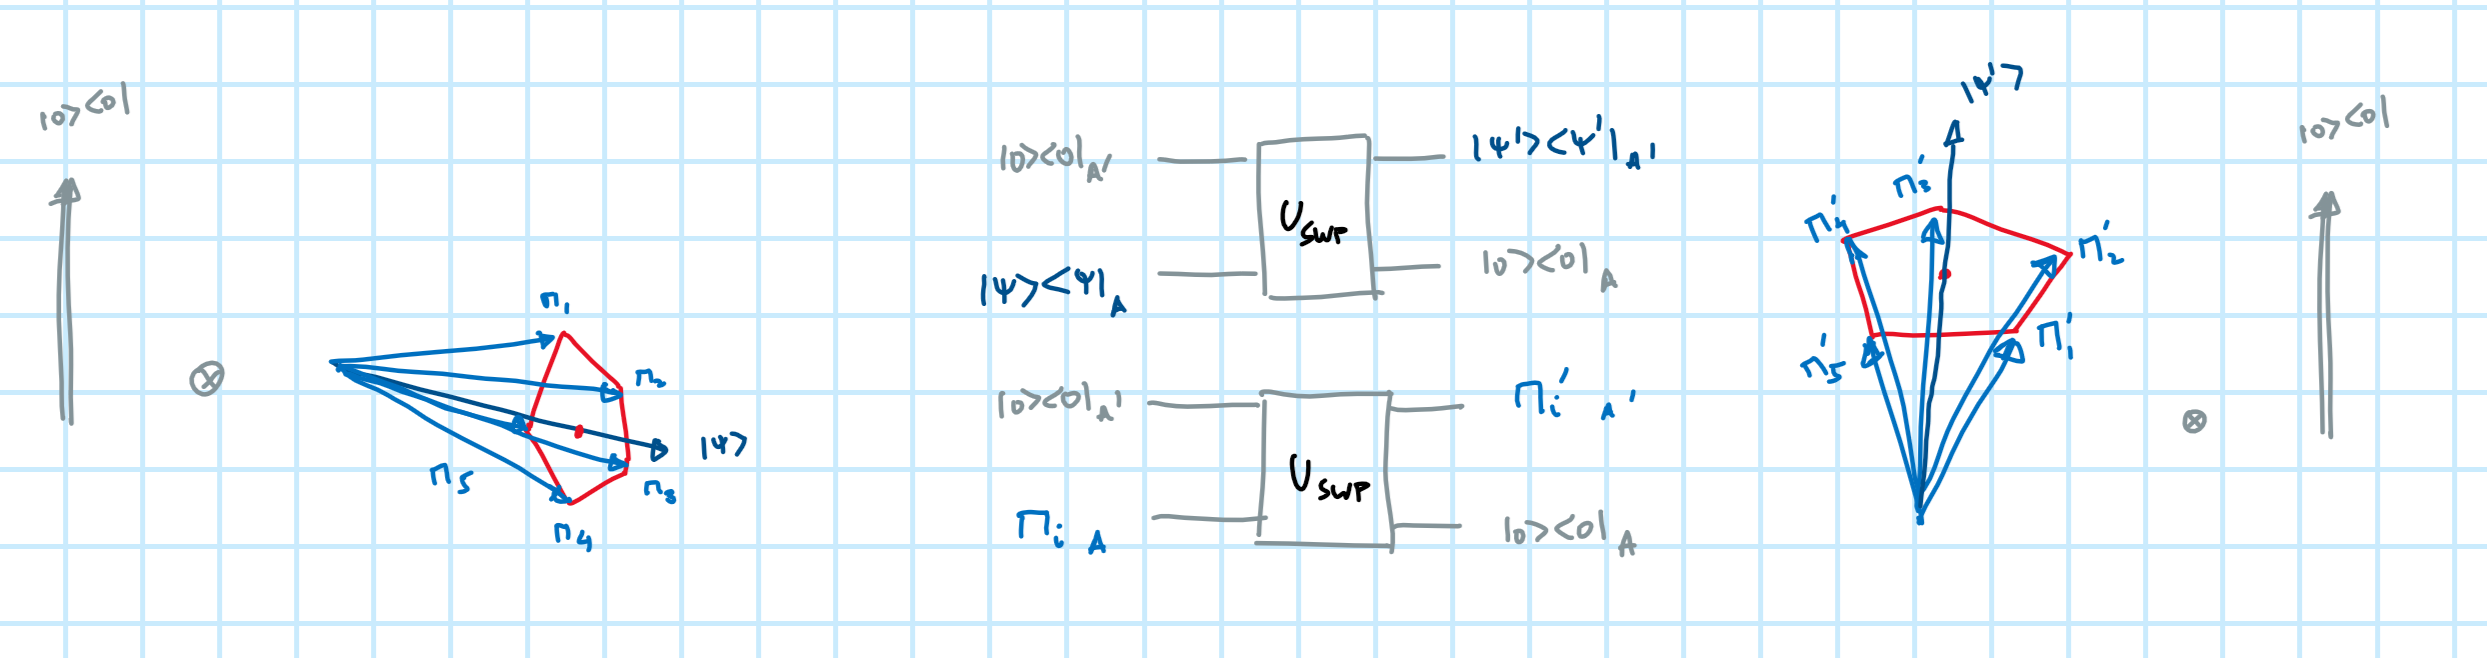
\includegraphics[width=0.7\paperwidth]{img/Isometry_temp}
\par\end{centering}
\caption{Illustration of $U_{\text{SWAP}}$.\label{fig:IllustrationSWAP}}
\end{figure}

We can now combine all the pieces to write the final optimisation
problem we solve. 
\begin{lyxalgorithm}[The SDP for lower bounding the fidelity of a given realisation with
the ideal KCBS realisation]
 The algorithm proceeds in two parts.\label{alg:The-algorithm} \\
\textbf{Notation:} Let
\begin{itemize}
\item $\mathcal{A}$ represent an arbitrary Hilbert space and $\mathcal{A}'$
represent a three dimensional Hilbert space,
\item $\bar{\mathcal{W}}$ be the set of ``words'' constructed using $\{\Pi_{i}\}_{i=1}^{5}$,
$\hat{P}$ and $\hat{P}^{\dagger}$, i.e. $\bar{\mathcal{W}}=\mathcal{G}(\{\Pi_{i}\}_{i=1}^{5},\hat{P},\hat{P}^{\dagger})$,
and 
\item define $\left\langle w\right\rangle :=\tr_{\mathcal{A}}(\rho w)$
and assume $\rho=\left|\psi\right\rangle \left\langle \psi\right|$
so that $\left\langle w\right\rangle =\left\langle \psi\right|w\left|\psi\right\rangle $
for all $w\in\mathcal{W}$.
\end{itemize}
\textbf{Input:}
\begin{itemize}
\item (implicit) $\Pi_{i}.\Pi_{j}=0$ for all $i,j\in E(G)$ where $G$
is a five cycle graph and $E$ are its edges, indexed $[1,2,\dots5]$
\item Expectation value of the KCBS operator: $\frac{1}{2}\sum_{i,j\in E(G)}\Pr[\Pi_{i}=1|\Pi_{j}=0]=:c$
\end{itemize}
\textbf{Evaluation | Part 1.}
\begin{itemize}
\item Evaluate $S_{\swap}$ as described in \Lemref{UswapIsAnIsometry}
using \Algref{ConstructingAnIsometry}. 
\item Define the objective function $f$ as 
\begin{align*}
f\left(\rho,\left\{ \Pi_{i}\right\} _{i=1}^{5}\right) & =\sum_{i=1}^{5}\mathcal{F}\left(\tr_{\mathcal{A}}\left[S_{\swap}\left(\Pi_{i}\rho_{\mathcal{A}}\Pi_{i}\otimes\left|0\right\rangle \left\langle 0\right|_{\mathcal{A}'}\right)S_{\swap}^{\dagger}\right],\Pi_{i}^{\KCBS}\rho_{\mathcal{A}'}^{\KCBS}\Pi_{i}^{\KCBS}\right)\\
 & \quad+\mathcal{F}\left(\tr_{\mathcal{A}}\left[S_{\swap}\left(\rho_{\mathcal{A}}\otimes\left|0\right\rangle \left\langle 0\right|_{\mathcal{A}'}\right)S_{\swap}^{\dagger}\right],\rho_{\mathcal{A}'}^{\KCBS}\right)
\end{align*}
and evaluate the coefficients $f_{w}$ so that 
\[
f=\sum_{w\in\mathcal{W}}f_{w}\left\langle w\right\rangle .
\]
\item Again, from \Algref{ConstructingAnIsometry}, evaluate $P_{\mathcal{A}}$
as a linear combination of $\left\langle w\right\rangle $. 
\end{itemize}
\textbf{Evaluation | Part 2.} Solve the following SDP. 
\begin{align*}
F_{\text{noiseless}}= & \min_{\{\left\langle w\right\rangle \}_{w\in\mathcal{W}}}\sum_{w\in\mathcal{W}}f_{w}\left\langle w\right\rangle \\
{\rm s.t.}\quad & \Gamma^{(k)}(\mathbb{I})\ge0 & \because\text{ all gram matrices are }\ge0\\
 & \Gamma^{(k)}(\mathbb{I})_{v,w}=\Gamma^{(k)}(\mathbb{I})_{v',w'} & \text{if }v^{\dagger}w=v^{\prime\dagger}w'\\
 & \Gamma^{(k)}(\hat{P}_{\mathcal{A}}P_{\mathcal{A}})\ge0 & \text{(localising matrix)}\\
 & \Gamma^{(k)}(\hat{P}_{\mathcal{A}}P_{\mathcal{A}})_{v,w}=\Gamma^{(k)}(\hat{P}_{\mathcal{A}}P_{\mathcal{A}})_{v',w'} & \text{if }v^{\dagger}\hat{P}_{\mathcal{A}}P_{\mathcal{A}}w=v^{\prime\dagger}\hat{P}_{\mathcal{A}}P_{\mathcal{A}}w'\\
 & \sum_{i=1}^{5}\left\langle \Pi_{i}\right\rangle =c & \text{(observed statistic)}
\end{align*}
where $\Gamma^{(k)}(X)$ is a matrix which is 
\begin{itemize}
\item indexed by letters $w$ 
\item whose matrix elements are given by $\Gamma^{(k)}(X)_{v,w}=\left\langle \psi\right|v^{\dagger}Xw\left|\psi\right\rangle $, 
\item where $k$ defines the maximum number of letters that appear in the
words $w$ which index the matrix $\Gamma^{(k)}$, and,
\end{itemize}
where in the first two equality constraints, we use the following
relations 
\begin{itemize}
\item $\Pi_{i}.\Pi_{j}=0$ for all $i,j\in E(G)$ and
\item $\hat{P}_{\mathcal{A}}^{\dagger}\hat{P}_{\mathcal{A}}=\hat{P}_{\mathcal{A}}\hat{P}_{\mathcal{A}}^{\dagger}=\mathbb{I}_{\mathcal{A}}$.
\end{itemize}
\textbf{Output:} $F_{\text{noiseless}}(c)$.
\end{lyxalgorithm}

\begin{rem}
Note that $\hat{P}P\ge0\implies\Gamma^{(k)}(\hat{P}P)\ge0$. This
follows readily by letting $A^{\dagger}A=\hat{P}P$ for some $A$
(which must exist for any positive semi-definite matrix; one can use
spectral decomposition). Then $\Gamma^{(k)}(A^{\dagger}A)$ is a gram
matrix and thus $\ge0$.
\end{rem}

\begin{rem}
TODO: explain why restricting to real $\left\langle \psi\right|w\left|\psi\right\rangle $
is enough.
\end{rem}

We thus have an algorithm which can calculate the required lower bound
on fidelity, given the observed value of the KCBS operator. In practice,
however, the assumption $\Pi_{i}.\Pi_{j}=0$ for all $i,j\in E(G)$
cannot be met. We discuss and remedy this next.

\section{Connection with the experiment}

\global\long\def\comp{\text{comp}}%

KISHOR: Move these things to the introduction/preliminaries as needed;
I am just writing these here to be consistent and clear.

\subsection{The Ideal Case}

We revisit the notion of exclusivity. Recall that we defined exclusivity
at the operational level---at the level of preparations and operations
(measurements are special cases with more than one outcome) which
in quantum theory correspond to states and unitary evolution (or measurements).
We said that two events $e_{1}$ and $e_{2}$ are exclusive if there
is some measurement $M$ for which the events correspond to different
outcomes of the measurement. To a set of events $\{e_{1},e_{2}\dots e_{5}\}$
we associated what we called an exclusivity graph, $G$, formed by
treating the events as vertices and their exclusivity relations as
edges. We defined a behaviour as a map from events to probabilities
such that $\Pr[e_{i}]+\Pr[e_{j}]\le1$ whenever $\left(i,j\right)\in E(G)$.
We defined non-contextual behaviours as those which admit a non-contextual
completion (details ...). We defined a quantum behaviour to be one
which can be realised using a quantum state and measurements. 
\begin{defn}[Quantum Behaviour]
 There exist projectors $\Pi_{i}$ associated with each event $e_{i}$
such that $\Pi_{i}.\Pi_{j}=0$ or equivalently $\tr(\Pi_{i}.\Pi_{j})=0$
whenever $\left(i,j\right)\in E(G)$ and that $\Pr[e_{i}]=\tr[\rho\Pi_{i}]$
for some fixed quantum state $\rho$ for each $i$. \label{def:quantumBehaviour}
\end{defn}

This we already knew. Let us now restrict to our case of interest,
the pentagonal exclusivity graph, i.e. the $5$-cycle graph. Observe
that the notion of exclusivity as defined does not exactly specify
the experimental arrangement---it only assigns projectors to certain
events but does not precisely specify the measurements which constitute
the events (only its existence is supposed). We now describe, again
at an operational level, one possible process which corresponds to
the pentagonal exclusivity graph. 
\begin{defn}[(Operational) KCBS process]
 Consider a preparation $\rho$ (we use quantum symbols to be suggestive)
and five measurements $\{\Pi_{i}^{\exp}\}_{i=1}^{5}$ with $0/1$
outcomes such that $\Pi_{i}^{\exp},\Pi_{i+1}^{\exp}$ are compatible
for $i\in\{1,2\dots5\}$; here the sum $i+1$ is modulo 5 plus 1.
We define 
\[
e_{i}:=(1,0|\Pi_{i}^{\exp},\Pi_{i+1}^{\exp})
\]
 that is the outcome is $1,0$ when $\Pi_{i}^{\exp}$ and $\Pi_{i+1}^{\exp}$
are measured. We call this process the \emph{KCBS process}. Denote
by $\Pr[e_{i}]$ the probability assigned to the event $e_{i}$ by
an appropriate probabilistic model and call $(\Pr[e_{i}])_{i}$ the
\emph{behaviour} corresponding to the KCBS process.\label{def:KCBS-process}
\end{defn}

\begin{rem}
Note, for instance, that $e_{1}$ and $e_{2}$ are indeed exclusive
because the outcome of measuring $\Pi_{2}^{\exp}$ is $0$ for $e_{1}$
and $1$ for $e_{2}$. 
\end{rem}

It is not hard to see (as we shall explicitly observe) that when this
KCBS process is governed by quantum theory, the resulting behaviour
is just the quantum behaviour for the pentagonal exclusivity graph.
We formally define quantum KCBS processes for clarity and state the
aforementioned as a lemma.
\begin{defn}[Quantum KCBS process]
 A KCBS process (see \Defref{KCBS-process}) where quantum theory
governs the probabilities, $\{\Pi_{i}^{\exp}\}_{i}$ are projectors
(not necessarily rank 1) and $\rho$ is a density matrix both defined
on an arbitrary but fixed Hilbert space.\label{def:KCBS-process-quantum}
\end{defn}

\begin{rem}
We could assume, without loss of generality, that the measurements
are projective (due to Naimark's theorem). However, even then, one
could not deduce that the $\Pr(1,1|\Pi_{1}^{\exp},\Pi_{1}^{\exp})=\tr(\Pi_{1}^{\exp}\Pi_{1}^{\exp}\rho\Pi_{1}^{\exp}\Pi_{1}^{\exp})$
because this would, in particular, entail that the measurement is
always repeatable which it needn't be. The theorem holds, but only
for one measurement; not sequential measurements as we require. Thus,
the quantum KCBS process as stated, is not the most general quantum
realisation of the KCBS process. In this article, we make this assumption
and leave its relaxation to future work. \label{rem:projectorsNaimarkInsufficient}
\end{rem}

\begin{lem}
The set of behaviours of quantum KCBS processes equals the set of
quantum behaviours for the pentagonal exclusivity graph.\label{lem:behaviourKCBSequalsQuantumBehaviour}
\end{lem}

\begin{proof}
We start with showing that every behaviour of a quantum KCBS process
can be cast as a quantum behaviour for the pentagonal exclusivity
graph. Define 
\[
\Pi_{i}:=\Pi_{i}^{\exp}(\mathbb{I}-\Pi_{i+1}^{\exp})\Pi_{i}^{\exp}
\]
so that $(\Pi_{i})_{i}$, $\rho$ define a quantum behaviour such
that 
\[
\Pr[e_{i}]=\tr[\rho\Pi_{i}]
\]
 as required. As a sanity check, note, for instance, that 
\begin{align*}
\Pi_{1}\Pi_{2} & =\Pi_{1}^{\exp}(\mathbb{I}-\Pi_{2}^{\exp})\Pi_{1}^{\exp}\Pi_{2}^{\exp}(\mathbb{I}-\Pi_{3}^{\exp})\Pi_{2}^{\exp}\\
 & =\Pi_{1}^{\exp}\cancelto{0}{(\mathbb{I}-\Pi_{2}^{\exp})\Pi_{2}^{\exp}}\Pi_{1}^{\exp}(\mathbb{I}-\Pi_{3}^{\exp})\Pi_{2}^{\exp}\\
 & =0
\end{align*}
because $[\Pi_{1}^{\exp},\Pi_{2}^{\exp}]=0$ (since the measurements
are compatible). 

We now show that every quantum behaviour can be realised as a quantum
KCBS process. Suppose the quantum behaviour is defined using $\left(\Pi_{i}\right)_{i},\rho$
and let $\Pi_{i}^{\exp}:=\Pi_{i}$. It follows that $(\Pi_{i}^{\exp})_{i},\rho$
define a quantum KCBS process because $[\Pi_{i}^{\exp},\Pi_{j}^{\exp}]=0$
for all $(i,j)\in E(G)$ (since $\Pi_{i}.\Pi_{j}=0$) where $G$ is
the pentagonal graph and $\tr(\rho\Pi_{i}^{\exp}(\mathbb{I}-\Pi_{i}^{\exp})\Pi_{i}^{\exp})=\tr(\rho\Pi_{i}^{\exp})=\Pr[e_{i}]$. 
\end{proof}
%
The analogous statement for the classical case also holds.
\begin{lem}
The set of behaviours of classical KCBS processes equals the set of
non-contextual behaviours for the pentagonal exclusivity graph.
\end{lem}

\begin{proof}
Idea: TODO: Kishor has to complete this; I hope it is trivial
\begin{itemize}
\item $[\Pi_{i}^{\exp},\Pi_{j}^{\exp}]=0$ for all $i,j\in V(G)$; $\left|\psi\right\rangle $
is arbitrary.
\item $\left|\psi\right\rangle $ s.t. $\Pi_{i}\left|\psi\right\rangle =\left|\psi\right\rangle $.
\end{itemize}
\end{proof}
To summarise, we defined the KCBS process to bridge the gap between
the exclusivity graph approach and the experiment being performed
in the lab. Note that both are, initially, defined at the operational
level. We saw that they give rise to the same set of classical and
quantum behaviours. The advantage of defining the KCBS process is
two-fold. (1) It moves us closer to a device independent description
and, as we shall see, (2) it facilitates the handling of experimental
imperfections insofar as the enforcement of the underlying assumptions
is concerned. {[}TODO: swap 1 and 2{]} It also clarifies that the
fidelity we calculate is for the abstract projectors $(\Pi_{i})_{i}$
which are related to, but not exactly equal to, the projectors $(\Pi_{i}^{\exp})_{i}$
which model the quantum KCBS process, i.e. the experiment (under the
sharpness assumption; see \Remref{projectorsNaimarkInsufficient}).

\subsection{Experimental Imperfections}

Two issues can plague an experimental realisation of a quantum KCBS
process (see \Defref{KCBS-process-quantum}). First, as already alluded
to in \Remref{projectorsNaimarkInsufficient}, the measurements may
not be exactly repeatable which means that one cannot assume them
to be projectors. In this work, we do not address this problem. Second,
the measurements may not be exactly compatible, which may manifest
as $p(a,b|x,y)$ being only approximately equal to $p(b,a|y,x)$.
In the following, we discuss one way of handling this imperfection. 

\subsection{SDP with non-orthogonal projectors}

TODO: Atul: I may have to reformulate this part because if we relax
the orthogonality condition, then it is no longer clear that the resulting
``isometry'' $S_{\swap}'$ is in fact an isometry. There are then
two steps; first, we have to show that the new objective (with the
noisy ...). 

Suppose we are given a quantum KCBS process (see \Defref{KCBS-process-quantum})
and to it we associate a quantum behaviour (see \Defref{quantumBehaviour})
as in the proof of \Lemref{behaviourKCBSequalsQuantumBehaviour},
i.e. we identify $\Pi_{i}=\Pi_{i}^{\exp}(\mathbb{I}-\Pi_{j}^{\exp})\Pi_{i}^{\exp}$.
We saw (again in the proof) that $[\Pi_{i}^{\exp},\Pi_{j}^{\exp}]=0\implies\Pi_{i}.\Pi_{j}=0$.
It is easy to see that $\left\Vert \Pi_{i}.\Pi_{j}\right\Vert _{2}\le\left\Vert [\Pi_{i}^{\exp},\Pi_{j}^{\exp}\right\Vert _{2}$
by using the triangle inequality and noting that $\left\Vert \Pi_{i}^{\exp}\right\Vert _{2}\le1$
(and the norm we use is the one induced by the vector norm). We now
lower bound the result of the SDP in \Algref{The-algorithm} when
the requirement $\Pi_{i}.\Pi_{j}=0$ is replaced with $\left\Vert \Pi_{i}.\Pi_{j}\right\Vert _{2}\le\epsilon$.
\begin{defn}
L\label{def:nonOSDP}et $F_{\text{nonO}}(c)$ be the output of \Algref{The-algorithm}
where ``Evaluation, part 2'' (the SDP part) is changed as follows
(by non-O we mean non-orthogonal).
\end{defn}

\begin{itemize}
\item The first equality constraint, $\Gamma^{(k)}(\mathbb{I})_{v,w}=\Gamma^{(k)}(\mathbb{I})_{v',w'}$
is imposed when $v^{\dagger}w=v^{\prime\dagger}w'$ as stated except
that we do not assume $\Pi_{i}.\Pi_{j}=0$.
\item Similarly, the second constraint, $\Gamma^{(k)}(\hat{P}_{\mathcal{A}}P_{\mathcal{A}})_{v,w}=\Gamma^{(k)}(\hat{P}_{\mathcal{A}}P_{\mathcal{A}})_{v',w'}$
is also imposed when $v^{\dagger}\hat{P}_{\mathcal{A}}P_{\mathcal{A}}w=v^{\prime\dagger}\hat{P}_{\mathcal{A}}P_{\mathcal{A}}w'$
as stated except that we do not assume $\Pi_{i}.\Pi_{j}=0$.
\end{itemize}
\begin{lem}
Let $F_{\text{noiseless}}(c)$ be the output of \Algref{The-algorithm}
on the input $c$ and let $F_{\text{nonO}}(c)$ be as described in
\Defref{nonOSDP}. Suppose $\left\Vert \Pi_{i}.\Pi_{j}\right\Vert _{2}\le\epsilon$. 
\end{lem}

We now obtain an expression for ... {[}{*}{*} I am here {*}{*}{]} 

\subsection{Towards a device independent perspective}

We attempt a rephrasing of the KCBS process in a device independent
language. 

\begin{figure}
\begin{centering}
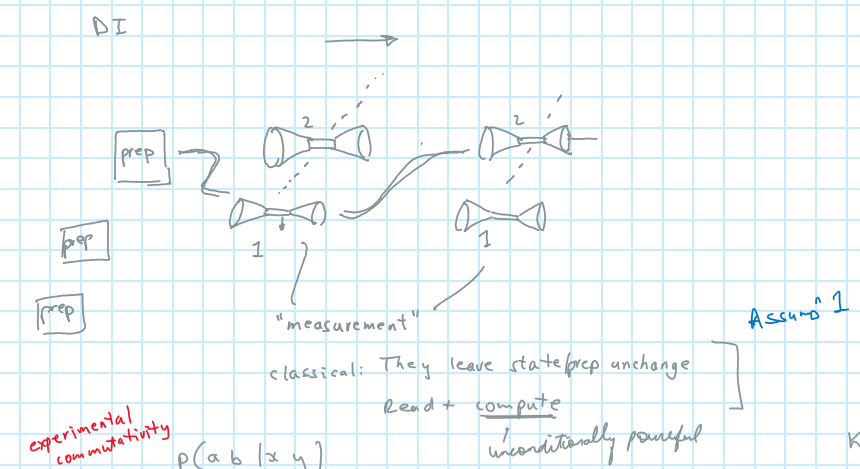
\includegraphics[width=0.7\textwidth]{img/KCBS_device}
\par\end{centering}
\caption{A KCBS Device\label{fig:The-KCBS-Device}}

\end{figure}

\begin{figure}
\begin{centering}
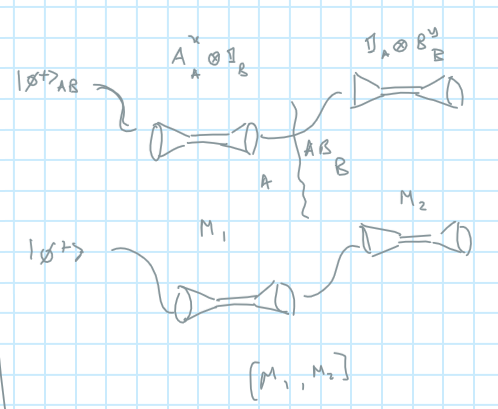
\includegraphics[width=0.4\textwidth]{img/KCBS_device_bell_like}
\par\end{centering}
\caption{Bell as a special case; allows for direct enforcement of the assumptions}

\end{figure}

\begin{defn}[A KCBS Device]
 An ($\epsilon,\delta$)--KCBS Device has three parts. 
\begin{enumerate}
\item[(i)] Input module (this is supposed to correspond to the preparation $\rho$).
\item[(ii)] Reader modules labelled ${\rm X}1,{\rm X}2\dots{\rm X}5,{\rm Y}1,{\rm Y2},\dots{\rm Y}5$
which when applied on an input module, output $0/1$ (these correspond
to the measurements $\left\{ \Pi_{i}\right\} _{i=1}^{5}$).
\end{enumerate}
The device takes as input an ordered pair $(x,y)\in\{1,2,\dots5\}\times\{1,2\dots5\}$
and returns two ordered bits $(a,b)$ generated by the following procedure.
\begin{enumerate}
\item The input module read using the reader module labelled $Xx$ and its
output is returned as $a$.
\item The input module is subsequently read using the reader module labelled
$Yy$ and its output is returned as $b$.
\end{enumerate}
Denote by $p(a,b|x,y)$ the probability (over identical copies of
the device) of obtaining the output $(a,b)$ given $(x,y)$ as the
input. The device satisfies, what we call the $(\epsilon,\delta)$
condition, i.e. 
\begin{align*}
\left|p(a,b|x,y)-p(b,a|y,x)\right| & \le\epsilon\quad\forall\:a,b\in\{0,1\}\quad\forall\:x,y\in\{1,2\dots5\}\\
\left|p(a,a|x,x)-p(a|x)\right| & \le\delta\quad\forall\:a\in\{0,1\}\quad\forall x\in\{1,2\dots5\}
\end{align*}
\emph{for all} possible input modules.
\end{defn}

A few remarks are in order. This definition is not very useful from
a device independent point of view as it is infeasible to imagine
that all possible input modules are tested. Further, we require a
device independent condition which, in quantum theory, should reduce
to the requirement that $(\Pi_{i}^{\exp})_{i}$ in fact behave like
measurements and in the classical case, should reduce to the requirement
that $\left(\Pi_{i}^{\exp}\right)_{i}$ do not influence the state
$\rho=\left|\psi\right\rangle \left\langle \psi\right|$ being measured
(we can then take convex combinations of these states).

\section{Experimental results}

The experimental implementation corresponding to the work in ref \cite{Bharti2018}
was carried on.

\section{Discussion}

\section{Conclusions}

\bibliographystyle{plain}
\bibliography{theta_number}

\end{document}
